
% This LaTeX was auto-generated from MATLAB code.
% To make changes, update the MATLAB code and republish this document.

\documentclass{article}
\usepackage{graphicx}
\usepackage{color}
\usepackage{amsmath}
\usepackage{amssymb}
\usepackage[a4paper, total={6in,8in}]{geometry}
\usepackage{pdfpages}

\sloppy
\definecolor{lightgray}{gray}{0.5}
\setlength{\parindent}{0pt}

\begin{document}


\includepdf{../TitlePage.pdf}

\hrulefill
\subsection*{Calculate final time}

\begin{par}
    From the equation of velocity in $r$ direction,
    \begin{equation}V_r = \frac{dr}{dt} \Rightarrow V_r dt = dr\end{equation}
    Integral both side,
    \begin{equation}\int^t_0 V_r dt = \int^{R_1}_{R_0} dr\end{equation}
\end{par}

\dotfill
\subsection*{Matlab program}
\begin{verbatim}
eqn_Vr = int(v, t, 0, t)-int(1, dr, R0, R1);
eqn_t = simplify(solve(eqn_Vr,t));

t_final = abs(subs(eqn_t, {R0 R1 a}, {R0n R1n an}));
\end{verbatim}

\hrulefill
\subsection*{Calculate the trajectory of the particle}

\begin{par}
    The equation of radius for the particle is
    \begin{equation}r(t) = R_0 + \int^t_0 V_r dt\end{equation}
    And the equation of direction for the particle is
    \begin{equation}\theta(t) = \theta_0 + \int^t_0 V_{\theta} dt\end{equation}
    where $V_{\theta} = \omega_0 = 0.05 \; \text{rad/s}$
\end{par}

\dotfill
\subsection*{Matlab program}
\begin{verbatim}
r = R0n + int(v,t);
theta = 0 + int(w,t);
tn = 0:0.01:t_final;
rn = subs(r, {a t}, {an, tn});
thetan = subs(theta, {t}, {tn});

polarplot(thetan,rn)
rlim([0 15])
title("The trajectory of the particle")
\end{verbatim}

\dotfill
\subsection*{Program result}
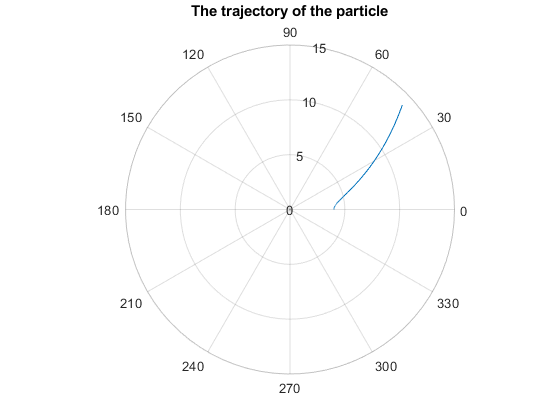
\includegraphics [width=4in]{HW2_01.png}

\begin{par}
    The result was not the same as the example in the textbook. In the textbook, the function input of the polar plot was using time(tn) and radius(rn). It is strange to use time value in the polar plot. The function input of the polar plot must be direction and radius. So I change the function input from time(tn) to direction(thetan).
\end{par}

\end{document}

